\documentclass[11pt]{article}

\usepackage[margin=1.1in]{geometry}
\usepackage{amsmath, amssymb}
\usepackage{graphicx}
\usepackage{booktabs}
\usepackage{microtype}
\usepackage{xcolor}
\usepackage[colorlinks=true, linkcolor=blue!50!black, urlcolor=blue!50!black]{hyperref}

\graphicspath{{figures/}}

\newcommand{\He}{\ensuremath{\heartsuit}}
\newcommand{\Sp}{\ensuremath{\spadesuit}}
\newcommand{\Di}{\ensuremath{\diamondsuit}}
\newcommand{\Cl}{\ensuremath{\clubsuit}}
\newcommand{\E}{\ensuremath{\mathbb{E}}}
\newcommand{\Prob}{\ensuremath{\mathbb{P}}}

\title{A Player's Guide to the Numbers:\\
\large statistics, probability, and game theory for our hearts-trump bidding game}
\author{Analysis notebooks 01--06 (\texttt{analysis/} in the hearts repo)}
\date{\today}

\begin{document}
\maketitle

\begin{abstract}
\noindent
We simulated millions of rounds of the game to answer the questions every
dedicated player eventually asks: how should I bid, does playing high or low
first matter, how bad is bidding last, is dealing first an advantage, and is
it worth counting cards? The short version: \textbf{bidding is worth an order
of magnitude more than card play}; the optimal bid follows a simple
probability threshold; the last-bidder constraint is a real, measurable tax;
first dealer in a two-player game wins a small edge---almost all of it in
round~1; and card counting pays handsomely, but \emph{only} through your
bids, because this game's deck is never reshuffled. Everything here assumes
college-level probability (expected value, distributions, confidence
intervals); nothing assumes more.
\end{abstract}

\tableofcontents

%=====================================================================
\section{The game, and the two rules that drive everything}
\label{sec:rules}

A quick formal recap, because two rules most players treat as flavor turn out
to control the entire analysis.

Each game has 13 rounds; round $r$ deals $c(r)$ cards to each player, with
$c(r)$ ramping $1,2,\dots,7,\dots,2,1$. Hearts are \emph{permanent trump}:
a heart beats any non-heart, higher hearts beat lower ones, and a card that
is neither trump nor the led suit can never win a trick, regardless of rank.
Each round, players bid the number of tricks they expect to win, dealer
first. A bid of $b$ with $t$ tricks actually won scores
\begin{equation}
\Delta(b, t) \;=\;
\begin{cases}
t + 1 & \text{if } t = b \quad\text{(made it exactly)},\\
-\,|b - t| & \text{otherwise.}
\end{cases}
\label{eq:score}
\end{equation}

The two load-bearing rules:

\begin{enumerate}
\item \textbf{The forbidden bid.} The last bidder may not choose a bid that
would make the round's bids sum to exactly $c(r)$ --- someone must be wrong.
This is a genuine constraint on one seat per round, and we can measure
exactly what it costs (\S\ref{sec:baseline}, \S\ref{sec:bidding}).
\item \textbf{The deck is shuffled once.} At the start of a game only. After
each round, the played cards go back \emph{under} the deck in the exact
public order they were played. Every card that leaves the deck is seen by
everyone, and its return position is determined by play order. The deck is
therefore not a randomizer after round~1 --- it is a conveyor belt, and a
sufficiently attentive player can read it (\S\ref{sec:tracking},
\S\ref{sec:counting}).
\end{enumerate}

\paragraph{How we measured things.} All results come from simulation against
a reference bot (``the heuristic'': bid $\approx$ your expected tricks from
hand strength, then play adaptively --- chase tricks while under your bid,
duck once you've made it). Where we compare two strategies we use
\emph{paired seeds}: both strategies play the exact same shuffled decks
against the exact same opponents, so their per-game score difference is a
low-variance estimate of the true gap. Error bars throughout are 95\%
confidence intervals; when we say an effect is ``real'' we mean its CI
excludes zero. A few small cases (one-card rounds) are solved
\emph{exactly}, by enumerating all deals --- no simulation error at all.

%=====================================================================
\section{Baseline: what the game looks like statistically}
\label{sec:baseline}

\begin{figure}[htbp]
\centering
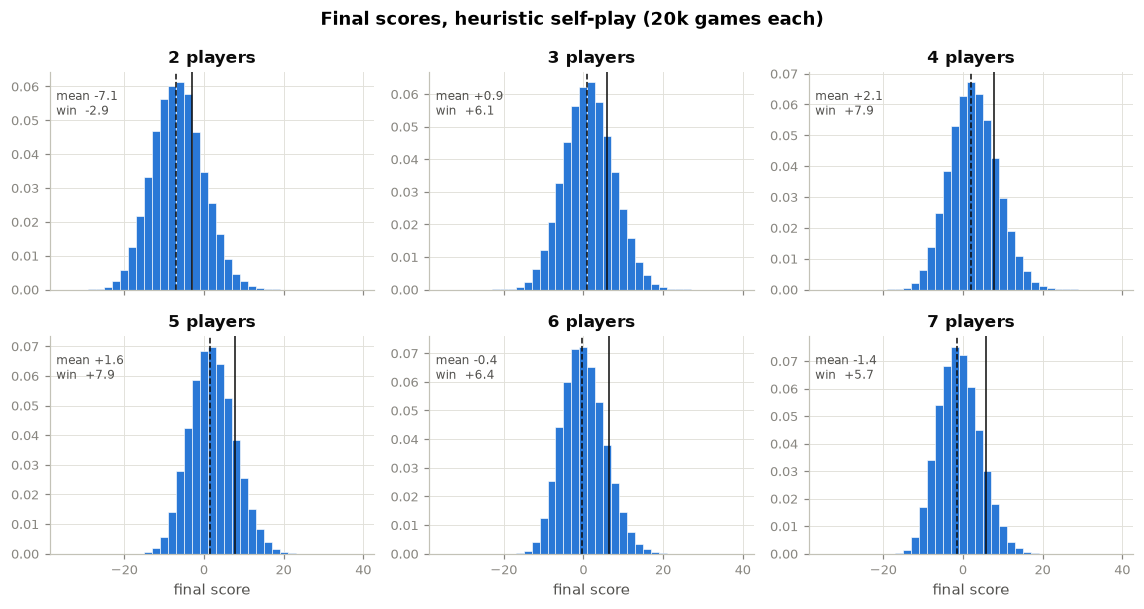
\includegraphics[width=\linewidth]{01_baseline_fig1.png}
\caption{Final-score distributions in heuristic self-play, 20{,}000 games
per table size. Dashed line: mean; solid line: mean \emph{winning} score.}
\label{fig:base-dist}
\end{figure}

Final scores are roughly bell-shaped with a standard deviation near 6 points
at every table size (Figure~\ref{fig:base-dist}). Mean score is not zero and
not constant: 4-player tables are the most generous ($+2.1$ per player on
average), heads-up is brutal ($-7.1$) --- with only two players, the
forbidden-bid rule binds on \emph{every} round (the last bidder is always
constrained), and misses are frequent. If your group plays for a running
total across evenings, be aware the table size changes the baseline.

\begin{figure}[htbp]
\centering
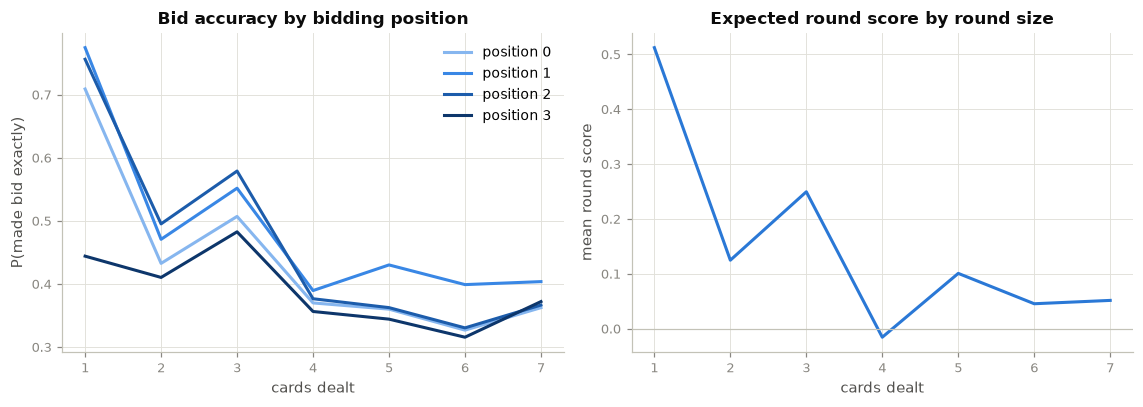
\includegraphics[width=\linewidth]{01_baseline_fig2.png}
\caption{Left: probability of making your bid exactly, by round size and
bidding position (4 players). Right: expected round score by round size.}
\label{fig:base-accuracy}
\end{figure}

Bid accuracy collapses as rounds grow (Figure~\ref{fig:base-accuracy}):
players hit a 1-card bid about $67\%$ of the time but a 6--7-card bid under
$38\%$. Since $\Delta$ rewards exactness, small rounds are where points are
reliably earned --- the expected round score falls from $+0.51$ in 1-card
rounds toward zero in big ones. \textbf{The 1-card rounds are not warm-ups;
per card dealt, they are the most valuable rounds in the game.}

\begin{figure}[htbp]
\centering
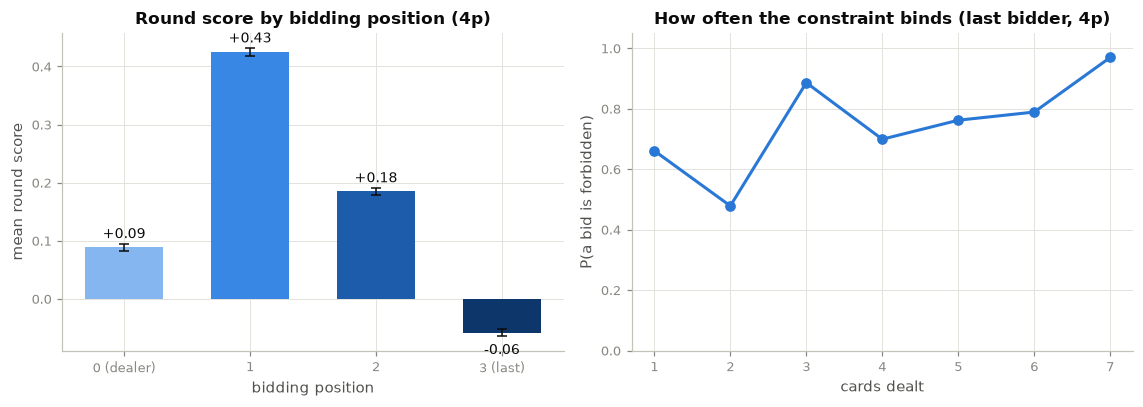
\includegraphics[width=\linewidth]{01_baseline_fig3.png}
\caption{Left: mean round score by bidding position at a 4-player table.
Right: how often the forbidden-bid constraint removes a bid the last bidder
might have wanted.}
\label{fig:base-tax}
\end{figure}

Position matters through the auction (Figure~\ref{fig:base-tax}). At four
players, bidding second is best ($+0.43$/round) and bidding \emph{last} is
worst ($-0.06$/round) even though the last bidder has the most information
--- the forbidden-bid rule more than cancels the informational advantage.
Call the gap the \emph{last-bidder tax}; at 4 players it runs about
$0.3$ points per round, and the constraint binds (removes a legal bid) in
$50$--$97\%$ of rounds depending on size. We compute this tax exactly in
\S\ref{sec:bidding}.

\begin{figure}[htbp]
\centering
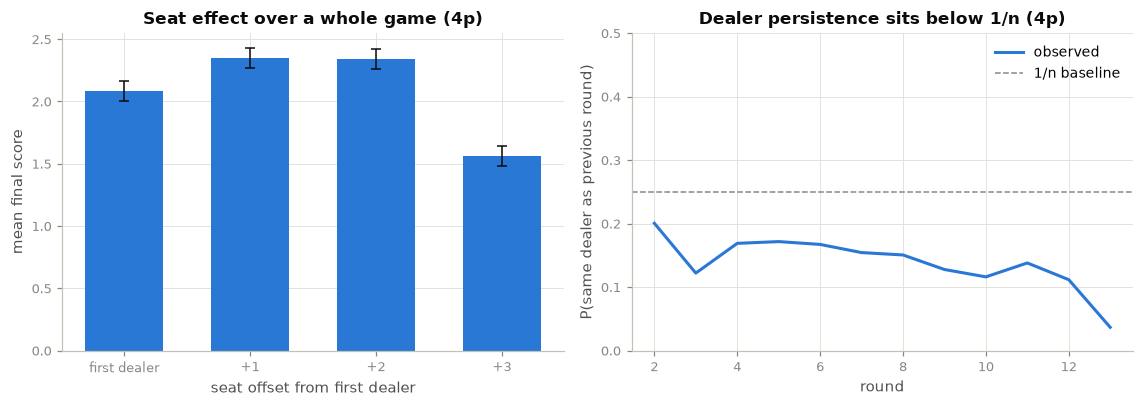
\includegraphics[width=\linewidth]{01_baseline_fig4.png}
\caption{Left: mean final score by seat, relative to the first dealer (4
players). Right: probability the same player deals twice in a row, versus
the $1/n$ baseline.}
\label{fig:base-seat}
\end{figure}

Two quieter structural facts (Figure~\ref{fig:base-seat}): seats one and two
to the left of the first dealer outscore the others over a full game
(they occupy the good bidding positions most often in the big middle
rounds), and \emph{dealer persistence} sits well below chance ($13.9\%$
versus $25\%$): the dealer of the next round is whoever won the last trick,
and the current dealer, having led the round's first trick, tends to have
spent their strength.

\begin{figure}[htbp]
\centering
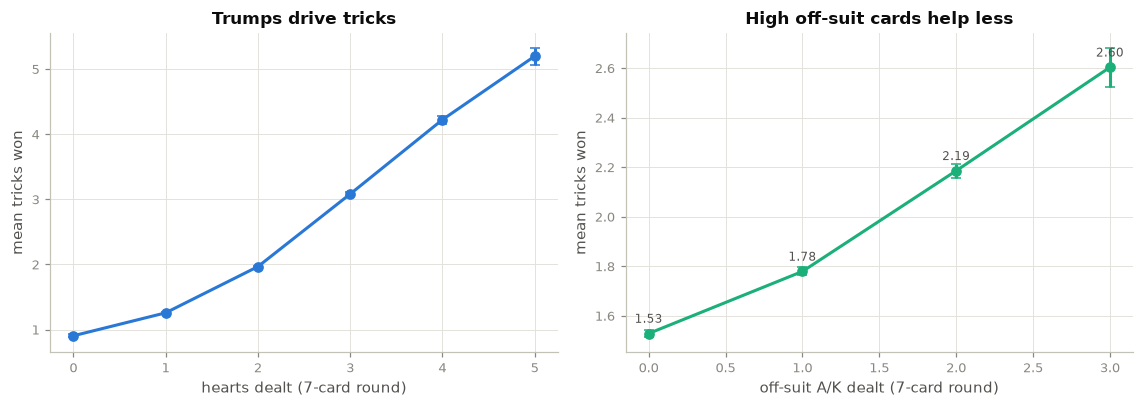
\includegraphics[width=\linewidth]{01_baseline_fig5.png}
\caption{Tricks won in the 7-card round as a function of hearts dealt
(left) and off-suit aces/kings dealt (right).}
\label{fig:base-drivers}
\end{figure}

\begin{figure}[htbp]
\centering
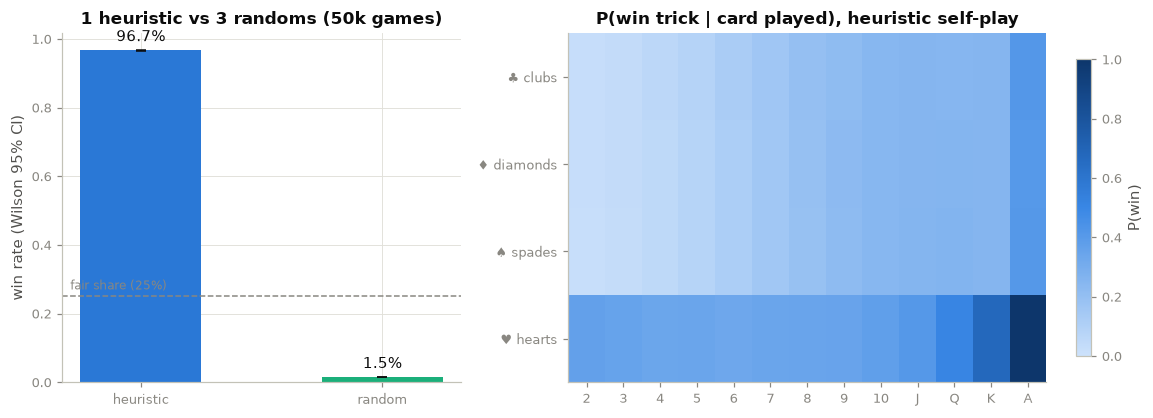
\includegraphics[width=\linewidth]{01_baseline_fig6.png}
\caption{Left: one heuristic bot at a table of three random bots wins
$96.7\%$ of games. Right: probability a played card wins its trick, by
suit and rank, in heuristic self-play.}
\label{fig:base-cards}
\end{figure}

What actually wins tricks? Hearts, overwhelmingly
(Figure~\ref{fig:base-drivers}): each heart dealt adds roughly one expected
trick ($\rho = 0.50$ between hearts dealt and tricks won), while off-suit
aces and kings add only fractions of a trick --- an off-suit ace still loses
to the two of hearts. The per-card view
(Figure~\ref{fig:base-cards}, right) is stark: the entire non-heart deck
wins at a fairly flat, low rate, and win probability only takes off inside
the trump suit. One number worth internalizing: the correlation between
tricks won and round score is \emph{negative} ($\rho = -0.14$). Tricks are
not points. Tricks you didn't bid for are anti-points.

Finally, the sanity check that play skill exists at all: one heuristic bot
among three random bots wins $96.7\%$ of games
(Figure~\ref{fig:base-cards}, left). ``Better than random'' is a low bar,
and the rest of this document is about the much narrower gaps between
sensible strategies.

%=====================================================================
\section{Bidding as a probability problem}
\label{sec:bidding}

\subsection{The 40\% rule}

Start with the smallest decision in the game: one card, bid 0 or 1. Let $p$
be the probability your card wins the trick. From Equation~\eqref{eq:score},
\[
\E[\Delta \mid \text{bid } 1] = 2p - (1-p) = 3p - 1,
\qquad
\E[\Delta \mid \text{bid } 0] = -p + (1-p) = 1 - 2p .
\]
Setting them equal: $3p - 1 = 1 - 2p$, so
\begin{equation}
p^\ast = \tfrac{2}{5} = 0.4 .
\label{eq:threshold}
\end{equation}
\textbf{Bid the trick if and only if you'd win it at least 40\% of the
time.} The threshold is below one-half because the payoff for a made bid of
1 (namely $+2$) exceeds the payoff for a made bid of 0 (namely $+1$): the
scoring pays you to take honest risks.

The win probability itself is a one-line hypergeometric computation. If $k$
of the other 51 cards beat yours (given that you lead, so your suit is the
led suit), then all $n-1$ opponents must draw from the $51-k$ harmless
cards:
\begin{equation}
\Prob(\text{win}) \;=\; \frac{\binom{51-k}{\,n-1\,}}{\binom{51}{\,n-1\,}} .
\label{eq:hyper}
\end{equation}

\begin{figure}[htbp]
\centering
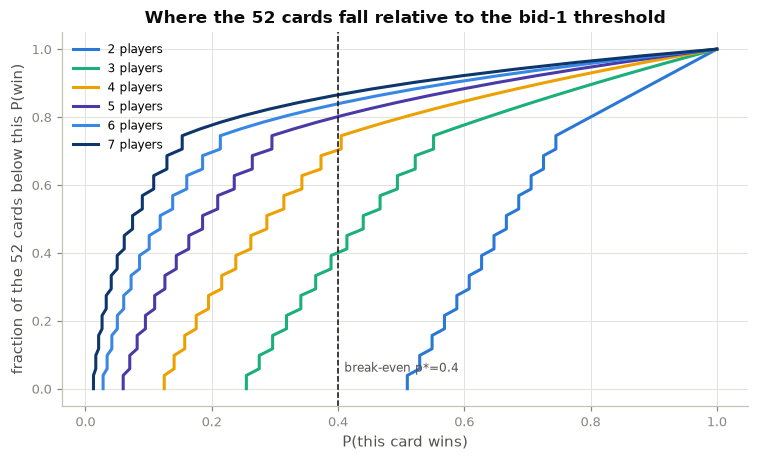
\includegraphics[width=0.9\linewidth]{04_equilibria_fig1.png}
\caption{Exact win probability of each of the 52 cards (led, round~1)
versus the bid-1 threshold $p^\ast = 0.4$, by table size.}
\label{fig:threshold}
\end{figure}

Figure~\ref{fig:threshold} evaluates \eqref{eq:hyper} for every card and
table size. Heads-up, \emph{every} card --- including the 2\Cl{} --- clears
the threshold: when you lead your only card against one opponent, even the
worst card wins just over half the time (the opponent's card is usually
off-suit and non-trump, and then it cannot win). Bid~1 on anything at two
players. At a full table of seven, only the top seven cards justify a bid.

\begin{figure}[htbp]
\centering
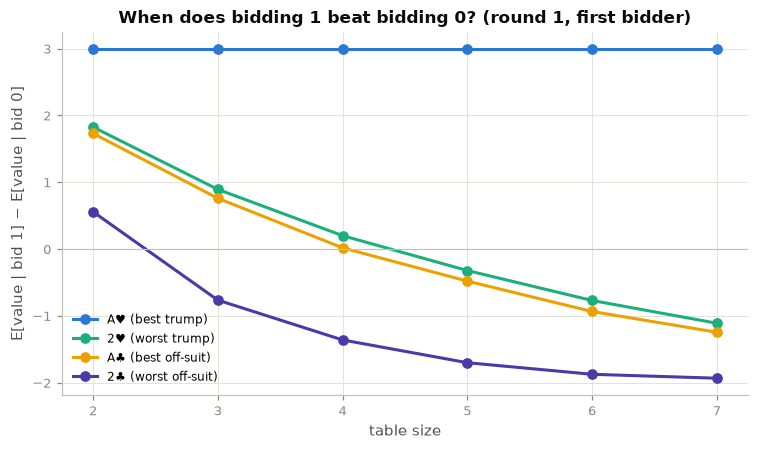
\includegraphics[width=\linewidth]{02_bidding_fig1.png}
\caption{Value of bidding 1 minus value of bidding 0 (round 1, first
bidder) for four reference cards, by table size.}
\label{fig:bid1vs0}
\end{figure}

\subsection{Bid tables for small rounds}

For 2- and 3-card rounds we estimated $\Prob(t \text{ tricks} \mid
\text{hand})$ by Monte Carlo (sampling opponent hands consistent with ours,
rolling the round out under a fixed greedy policy) and chose
$\arg\max_b \E[\Delta(b, T)]$. The resulting policy compresses to something
you can use at the table (Figure~\ref{fig:bidtables}): \textbf{in small
rounds, bid your hearts} --- with the notable exception that a single
\emph{low} heart in a 3-card round is a bid-0 hand, not a bid-1 hand
(one low trump wins a trick less than 40\% of the time once six other
cards are in play).

\begin{figure}[htbp]
\centering
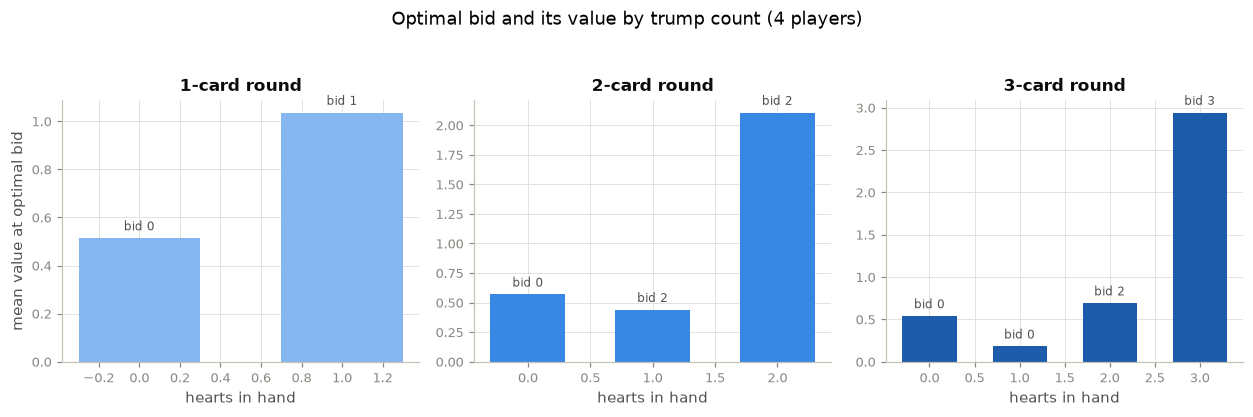
\includegraphics[width=\linewidth]{02_bidding_fig2.png}
\caption{Monte-Carlo optimal bid and its expected value by number of hearts
held (4 players).}
\label{fig:bidtables}
\end{figure}

\subsection{The last-bidder tax, exactly}

For 1-card rounds we can price the forbidden-bid rule with no simulation:
for each card and table size, compare the last bidder's expected score with
and without the constraint, averaging over all deals.
Figure~\ref{fig:exacttax} shows the result: about $0.36$ points per 1-card
round heads-up, $0.12$--$0.32$ elsewhere. It is worst at two players
because with one opponent the constraint binds every round and frequently
forbids precisely the bid the threshold rule wants.

\begin{figure}[htbp]
\centering
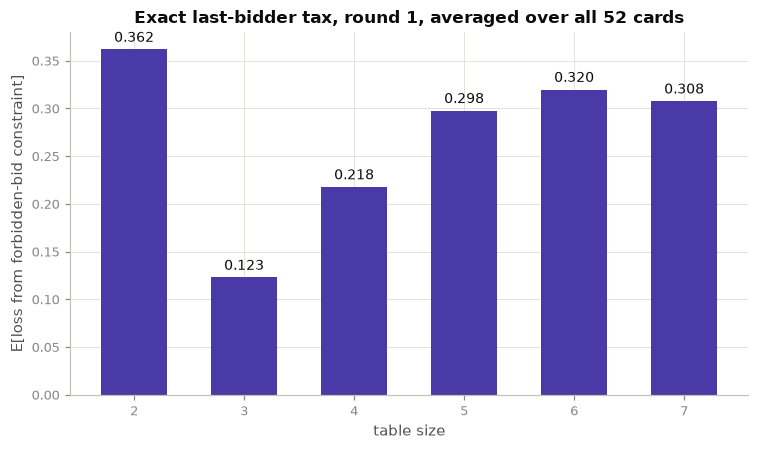
\includegraphics[width=0.8\linewidth]{02_bidding_fig3.png}
\caption{Exact expected loss inflicted on the last bidder by the
forbidden-bid rule, 1-card rounds.}
\label{fig:exacttax}
\end{figure}

\subsection{Does better bidding actually win games?}

Replacing the heuristic's hand-strength bid with the Monte-Carlo optimal
bid --- play unchanged --- lifts mean final score from $+2.27$ to $+2.95$
and win rate from $25.1\%$ to $29.1\%$ at a 4-player table
(Figure~\ref{fig:mcvsheur}). Two-thirds of a point per game from bidding
alone, before any card-play improvement. Hold that number against
\S\ref{sec:strategies}, where entire play styles are worth less.

\begin{figure}[htbp]
\centering
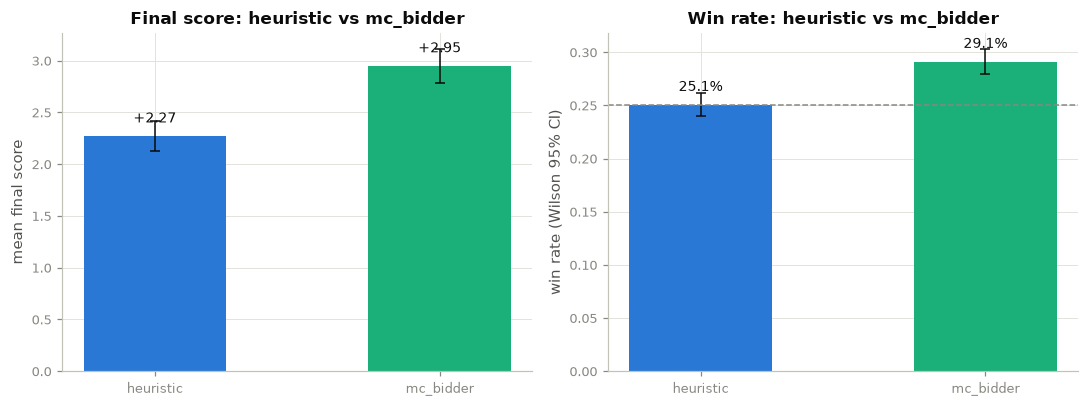
\includegraphics[width=\linewidth]{02_bidding_fig4.png}
\caption{Monte-Carlo bidder versus heuristic bidder, identical play policy,
4-player tables.}
\label{fig:mcvsheur}
\end{figure}

%=====================================================================
\section{The deck is an open book}
\label{sec:tracking}

Recall rule 2 of \S\ref{sec:rules}: one shuffle per game, played cards
returned to the bottom in play order. Consequence: once the game has dealt
more than 52 cards in total, every card being dealt is a card whose
position you could have derived from public information.

\begin{figure}[htbp]
\centering
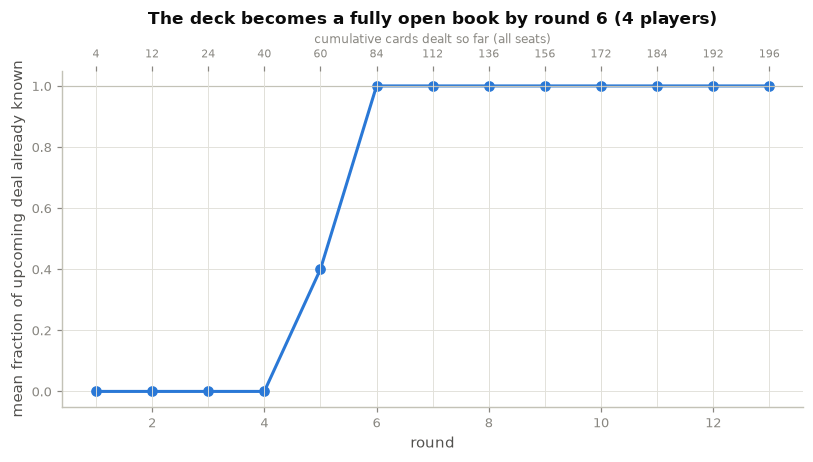
\includegraphics[width=0.95\linewidth]{03_deck_tracking_fig1.png}
\caption{Fraction of the upcoming deal that is fully determined by public
history, by round (4 players). The top axis counts cumulative cards dealt;
the jump happens exactly when it passes 52.}
\label{fig:infocurve}
\end{figure}

At a 4-player table the arithmetic is exact (Figure~\ref{fig:infocurve}):
rounds 1--4 deal $4+8+12+16 = 40$ cards off the fresh shuffle (nothing
knowable), round 5 needs 20 more but only 12 remain unseen --- so $40\%$ of
round 5's deal is publicly derivable --- and from round 6 onward
\textbf{every deal, including every opponent's exact hand, is 100\%
determined by cards everyone has already seen}. This is symmetric
information: it holds for every seat equally. The skill is bookkeeping, not
espionage.

\begin{figure}[htbp]
\centering
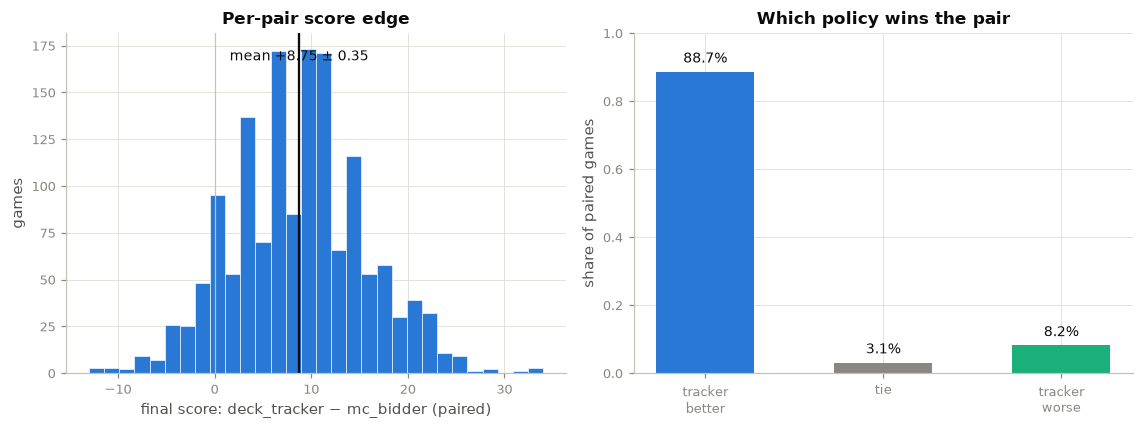
\includegraphics[width=\linewidth]{03_deck_tracking_fig3.png}
\caption{Paired-seed comparison, 1{,}500 games: a perfect deck tracker
versus an otherwise-identical Monte-Carlo bidder. Left: distribution of the
per-game score difference. Right: who wins each pair.}
\label{fig:trackeredge}
\end{figure}

How much is it worth? We gave one bot a perfect deck model feeding its bid
estimates (opponent cards it can foresee are fixed rather than sampled) and
left its card play identical to the baseline. On paired seeds the tracker
scores $+8.75$ points per game more (95\% CI $[8.41, 9.10]$) and is the
better of the pair in $88.7\%$ of games (Figure~\ref{fig:trackeredge}).
For scale: that dwarfs every other effect in this document. If your table
allows written notes, this is the game. If it doesn't,
\S\ref{sec:counting} prices the human-memory versions.

%=====================================================================
\section{Game theory: is the auction actually interactive?}
\label{sec:gametheory}

Bidding \emph{feels} interactive --- you see earlier bids before choosing
yours. For 1-card rounds we can settle exactly how much interaction is
real. With three players, the two free bidders (the third is forced by the
forbidden-bid rule) define a $2 \times 2$ game whose payoffs we computed by
enumerating all $52 \cdot 51 \cdot 50$ deals (Figure~\ref{fig:bimatrix}).

\begin{figure}[htbp]
\centering
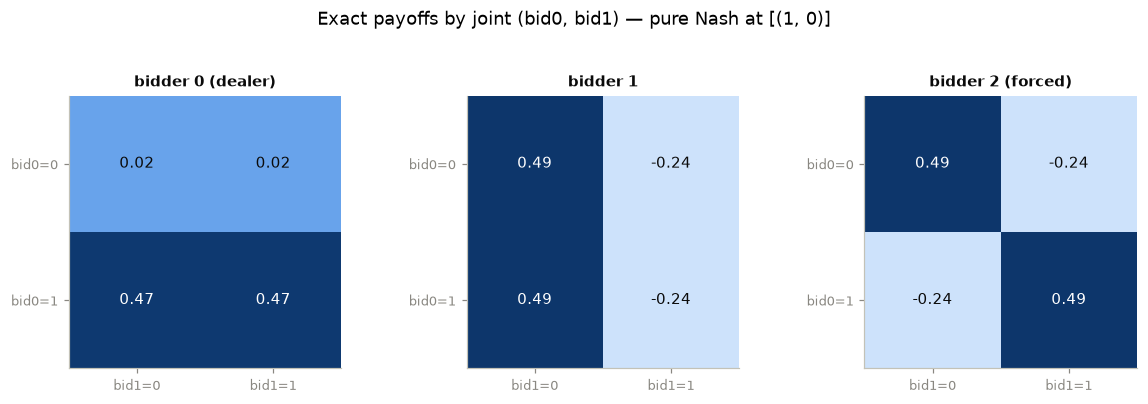
\includegraphics[width=\linewidth]{04_equilibria_fig2.png}
\caption{Exact expected payoffs in the 3-player 1-card round, by the two
free bids. Each free bidder's payoff is constant across the other's choice:
both have dominant strategies, with pure Nash equilibrium at
$(\text{bid}_0, \text{bid}_1) = (1, 0)$.}
\label{fig:bimatrix}
\end{figure}

The matrices have a striking property: each bidder's payoff is
\emph{constant} across the other's bid. Your bid cannot change who wins the
trick --- only the cards do that --- so in a 1-card round your optimal bid
is a pure statistics problem, not a psychology problem. The equilibrium is
$(1, 0)$: the dealer, who leads, should bid~1 (a led card always contends,
winning about 49\% of these rounds); the second bidder should bid~0. The
only player whose fate depends on others is the forced last bidder ---
interaction in this auction exists, but it is entirely concentrated in the
constraint, not in the choices.

\begin{figure}[htbp]
\centering
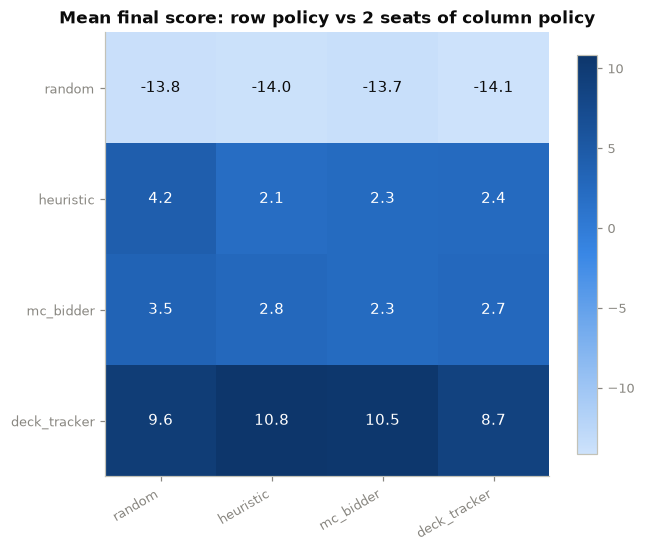
\includegraphics[width=0.7\linewidth]{04_equilibria_fig3.png}
\caption{Empirical meta-game: mean final score of the row policy at a
4-player table with two seats of the column policy, 800 games per cell.}
\label{fig:metagame}
\end{figure}

\begin{figure}[htbp]
\centering
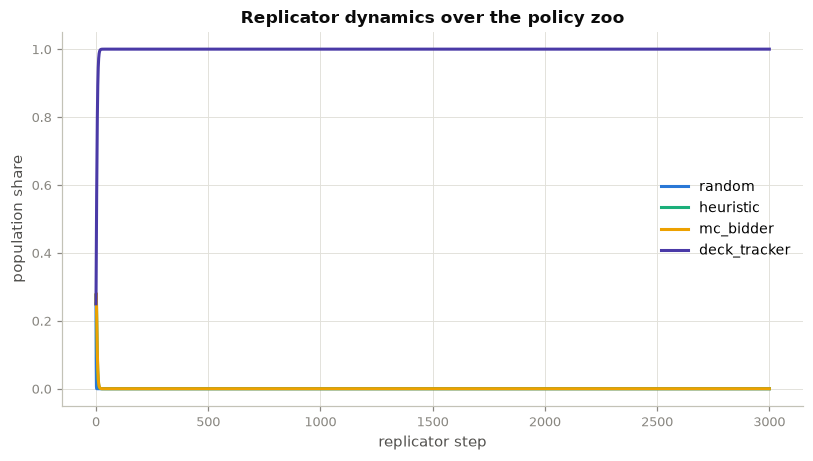
\includegraphics[width=0.85\linewidth]{04_equilibria_fig4.png}
\caption{Replicator dynamics over the four-policy meta-game: the deck
tracker takes over the population from a uniform start.}
\label{fig:replicator}
\end{figure}

Zooming out to whole games, we played every pairing of \{random, heuristic,
Monte-Carlo bidder, deck tracker\} (Figure~\ref{fig:metagame}) and ran
replicator dynamics on the resulting meta-game --- a standard model where
strategies ``reproduce'' in proportion to how well they score against the
current population mix. The deck tracker's row dominates every column,
including its own, and its population share goes to $1$
(Figure~\ref{fig:replicator}). There is no rock--paper--scissors structure
here: information is simply better than no information, transitively.

%=====================================================================
\section{Strategy families: what should a human actually do?}
\label{sec:strategies}

The optimal policies above are computational. This section tests
\emph{human-usable} rules: linear bidding formulas over hand features, and
fixed card-play orderings --- each varied while everything else is held
constant, on paired seeds.

\subsection{Bidding by formula}

A feature bidder computes $\hat{t} = \sum_i w_i f_i(\text{hand})$ over
features you can count at a glance --- hearts, high hearts (9+), off-suit
aces/kings, face cards --- and bids the nearest legal integer.

\begin{figure}[htbp]
\centering
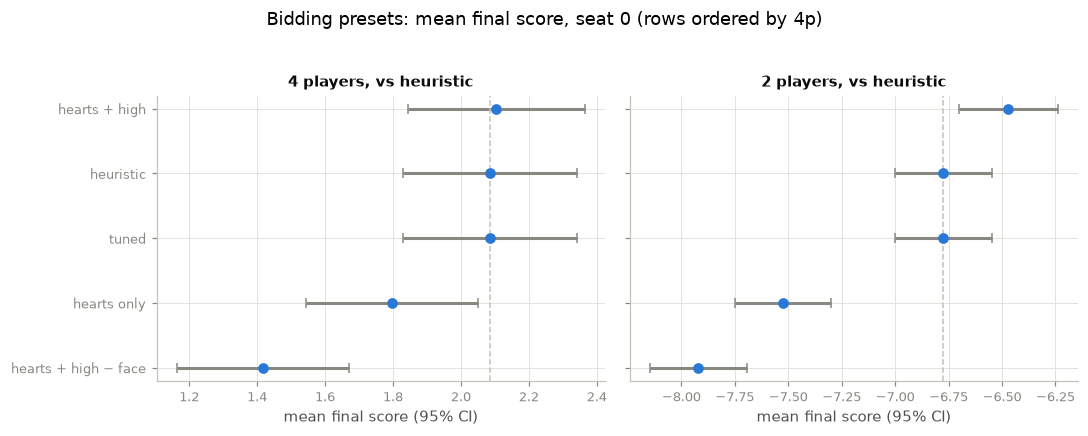
\includegraphics[width=\linewidth]{05_strategies_fig1.png}
\caption{Named bidding formulas, mean final score on identical games.
``tuned'' is algebraically identical to the reference heuristic and lands
exactly on it --- a built-in consistency check.}
\label{fig:presets}
\end{figure}

\begin{figure}[htbp]
\centering
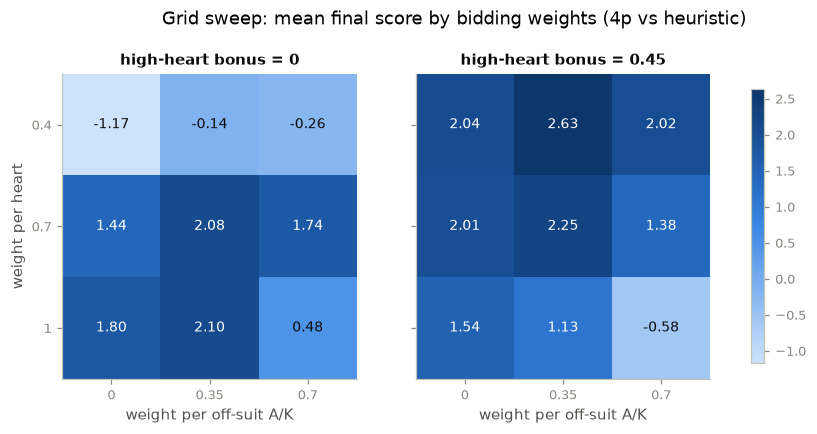
\includegraphics[width=0.95\linewidth]{05_strategies_fig2.png}
\caption{An 18-point sweep over the three load-bearing weights
(4 players, 2{,}000 games per point).}
\label{fig:grid}
\end{figure}

Findings (Figures~\ref{fig:presets} and \ref{fig:grid}):

\begin{itemize}
\item \textbf{``Bid your hearts'' captures most of the value.} Everything
sensible lives within about one point per game; for contrast, random
bidding is 16 points worse.
\item \textbf{Do not penalize face cards.} The
$\text{hearts} + \text{high} - \text{face}$ formula was the worst preset at
both table sizes. An off-suit king is a mild asset, not a trap.
\item \textbf{Underbid.} The best weights discount hearts steeply (0.4 per
heart, plus a bonus for hearts 9+) --- significantly better than the
reference weights by $+0.55 \pm 0.30$ per game. The logic: a miss costs
$|b - t|$ in either direction, but low bids are \emph{reachable} --- you
can duck your way down to a low bid, while a high bid needs the tricks to
actually materialize.
\item Off-suit aces and kings are worth about $0.35$ tricks in the formula:
more than zero, much less than a heart.
\end{itemize}

\subsection{Play styles, position, and phases}

Fixing the bid rule and varying only card play: \texttt{hearts\_first}
(dump trump early), \texttt{high\_first}, \texttt{low\_first}, and the
adaptive baseline (chase tricks while under bid, duck after), plus
phase-switching hybrids at both timescales (switching by round of the game,
or by trick within the round).

\begin{figure}[htbp]
\centering
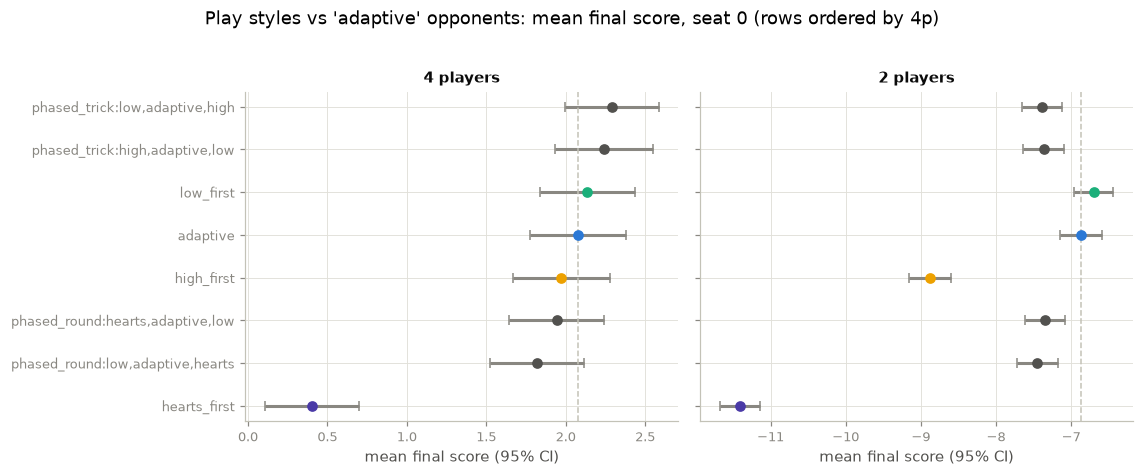
\includegraphics[width=\linewidth]{05_strategies_fig3.png}
\caption{Play styles on identical games, bidding held fixed. Note the
horizontal scale relative to Figure~\ref{fig:presets}: play styles move
scores far less than bidding formulas do.}
\label{fig:styles}
\end{figure}

\begin{figure}[htbp]
\centering
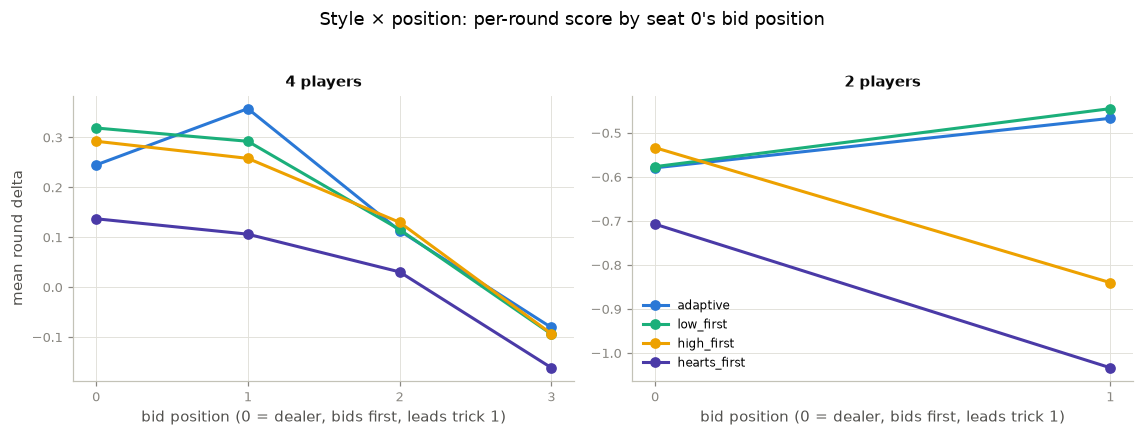
\includegraphics[width=\linewidth]{05_strategies_fig4.png}
\caption{Style $\times$ bidding position. At 4 players the curves are
parallel (position changes your score, not your best style); heads-up,
aggressive high-card play is only viable from the dealer's (leader's)
seat.}
\label{fig:styleposition}
\end{figure}

\begin{figure}[htbp]
\centering
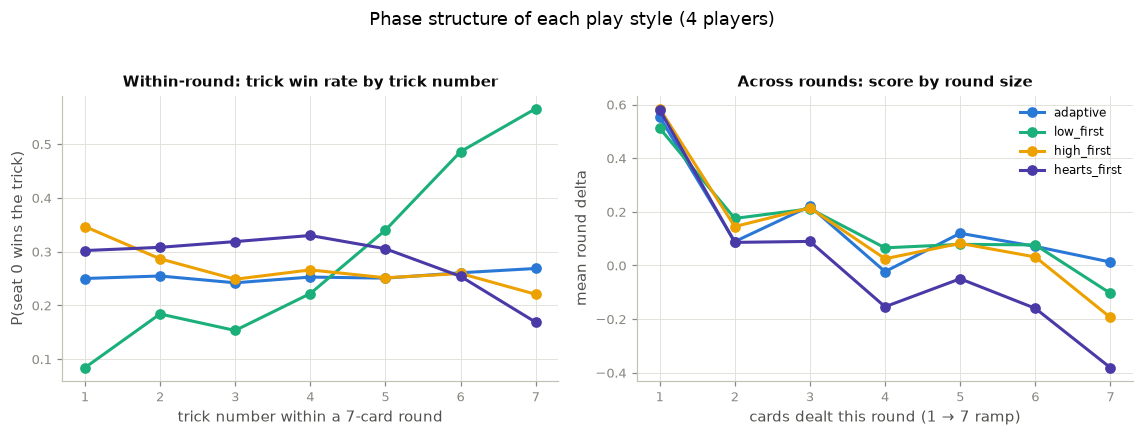
\includegraphics[width=\linewidth]{05_strategies_fig5.png}
\caption{Phase structure, 4 players. Left: when each style wins its tricks
within the 7-card round. Right: mean round score by round size.}
\label{fig:phases}
\end{figure}

Findings (Figures~\ref{fig:styles}--\ref{fig:phases}):

\begin{itemize}
\item \textbf{Play style is a $\pm 1$--$2$ point decision} --- an order of
magnitude smaller than bidding. Get the bid right first.
\item \textbf{Never lead with your hearts to ``get them out''.}
\texttt{hearts\_first} is by far the worst style at every table size
($-1.7$/game at 4 players, $-4.5$ heads-up). Trump is trick \emph{control};
spending it early is spending your steering wheel.
\item \textbf{\texttt{low\_first} is an excellent lazy default}, matching
or beating the adaptive baseline. Most bids are low, and playing low avoids
the accidental tricks that turn into $-1$s. Its trick-winning profile
(Figure~\ref{fig:phases}, left) is exactly what you want: it loses the
early tricks and wins the late ones, when winning is more often
intentional.
\item \textbf{Phases: round size is the axis that matters.} All styles
earn in the small rounds and bleed in the 5--7-card rounds, and the gaps
between styles widen with round size; switching styles \emph{within} a
round (by trick number) never significantly beat just playing the better
style throughout.
\item \textbf{Position mostly doesn't change your best style} (4 players:
parallel curves). The heads-up exception is worth knowing: high-aggression
play works only when you are the leader --- your led card always contends
--- and backfires as the follower.
\end{itemize}

\subsection{The first-dealer edge, heads-up}

Two identical bots, 20{,}000 games, seat 0 always dealing first: seat 0
scores $+0.30 \pm 0.15$ per game more (random-play control: $+0.17 \pm
0.17$). Small but real --- and the decomposition
(Figure~\ref{fig:dealeredge}, right) is the interesting part:
\textbf{essentially the whole edge is earned in round 1}. That is the only
round dealt from a genuinely uniform shuffle, and its single trick is led
by the dealer --- the purest form of the leader's structural advantage
(\S\ref{sec:gametheory}). From round 2 onward, deals come off the recycled,
play-ordered deck and the per-round dealer effect nets out to zero. If you
cut for first deal, you are cutting for the right to lead one clean coin
flip at favorable odds.

\begin{figure}[htbp]
\centering
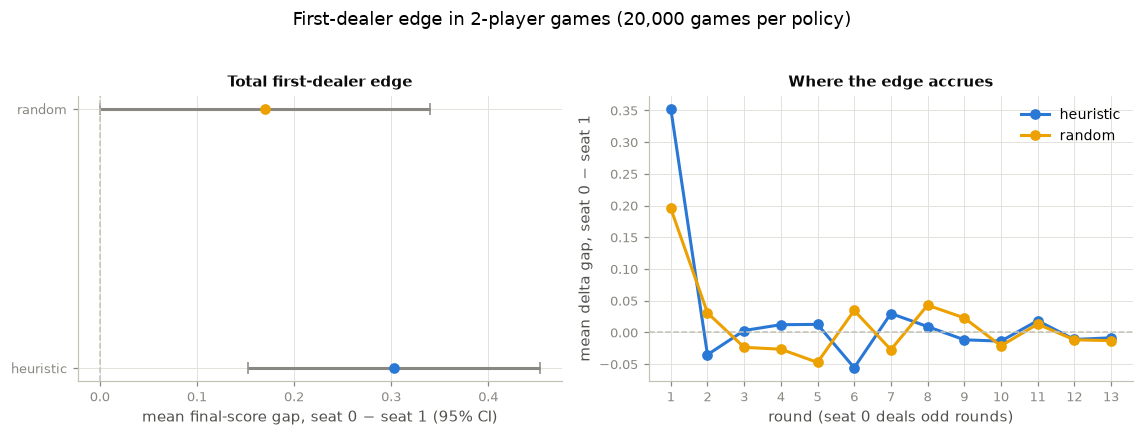
\includegraphics[width=\linewidth]{05_strategies_fig6.png}
\caption{First-dealer edge in 2-player games. Left: total edge (95\% CI).
Right: per-round decomposition --- the edge lives in round 1.}
\label{fig:dealeredge}
\end{figure}

\begin{figure}[htbp]
\centering
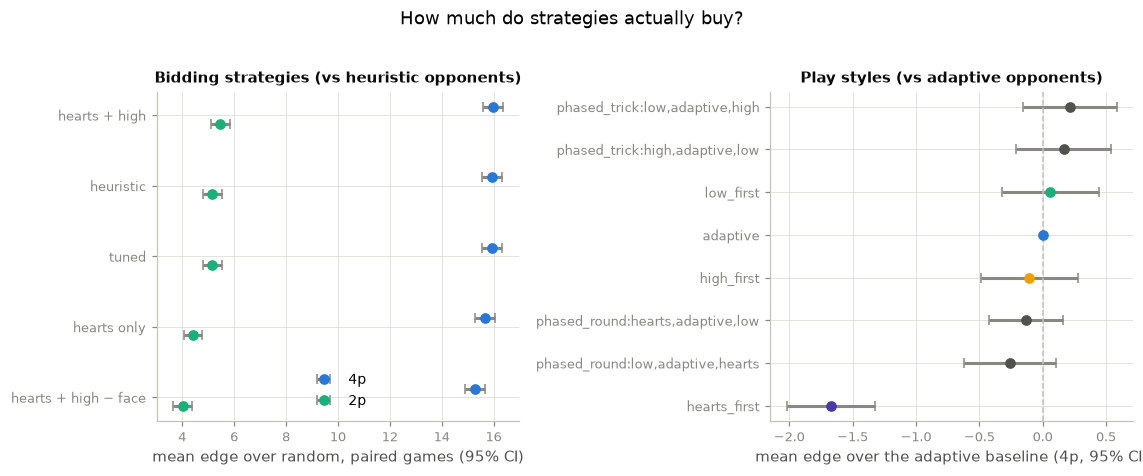
\includegraphics[width=\linewidth]{05_strategies_fig7.png}
\caption{The dominance chart: paired-seed edge of each bidding formula
over random (left) and of each play style over the adaptive baseline
(right).}
\label{fig:dominance}
\end{figure}

Figure~\ref{fig:dominance} assembles the hierarchy in one view. Against
random play, any sensible strategy is worth $+4$ to $+6$ points heads-up
and $+15$ to $+16$ at four players; the differences among sensible
strategies are the remaining $\pm 1$.

%=====================================================================
\section{Card counting: what is each level of memory worth?}
\label{sec:counting}

Perfect deck tracking is worth $+8.75$ (\S\ref{sec:tracking}), but nobody
remembers 52 card positions at the kitchen table. We graded the memory:

\begin{center}
\begin{tabular}{ll}
\toprule
level & what you remember \\
\midrule
\texttt{hearts\_count} & only \emph{how many} hearts have been played \\
\texttt{hearts\_exact} & \emph{which} hearts have been played \\
\texttt{high\_cards} & which of the 12 trick-deciders (off-suit A/K, hearts 9+) \\
\texttt{full} & everything (the \S\ref{sec:tracking} tracker) \\
\bottomrule
\end{tabular}
\end{center}

\noindent
and, crucially, ablated \emph{where} the memory is used: the \textbf{bid
channel} (memory of past rounds partially predicts future deals, because
the deck recycles deterministically) versus the \textbf{play channel}
(within a round, prefer the cheapest card whose survival probability
against the still-unseen cards clears a confidence threshold --- a
hypergeometric computation like Equation~\eqref{eq:hyper}, where memory
shrinks the threat pool). Each combination was measured on 1{,}500 paired
games against a baseline matched on everything except the memory.

\begin{figure}[htbp]
\centering
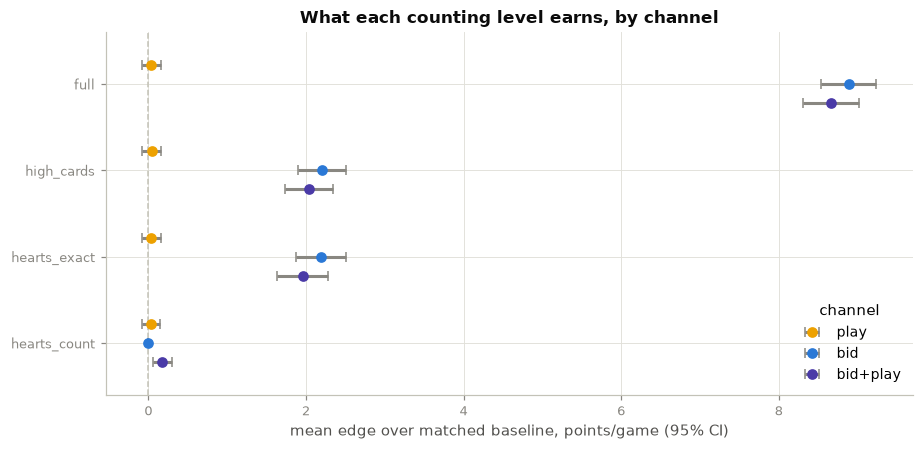
\includegraphics[width=0.95\linewidth]{06_counting_fig1.png}
\caption{Points per game earned by each memory level, by channel. All the
value flows through bidding.}
\label{fig:ladder}
\end{figure}

Findings (Figure~\ref{fig:ladder}):

\begin{itemize}
\item \textbf{Count for your bids, not your plays.} The bid channel earns
$+2.2$/game from realistic memory and $+8.9$ from perfect memory. The play
channel earns $\approx 0$ at \emph{every} memory level.
\item \textbf{Identities beat quantities.} Knowing \emph{how many} hearts
are gone earns exactly zero through bids --- a count cannot tell you which
seat is about to receive which card. Knowing \emph{which} hearts are gone
earns $+2.2$.
\item \textbf{Track winners, not suits.} Remembering the 12 trick-deciding
high cards ties remembering the entire 13-card trump suit ($+2.20$ vs
$+2.19$). Memory should chase the cards that decide tricks.
\end{itemize}

Why is within-round counting worthless? Not because the logic never fires
--- instrumenting 200 games shows about five ``I want this trick and have a
choice'' leads per game, and the confidence rule triggers regularly. The
reason is structural: at a 4-player table even the biggest round deals only
28 of 52 cards, and a within-round counter cannot distinguish ``not yet
played'' from ``never dealt.'' The unseen pool is dominated by cards
nobody holds, so remembering the handful actually played barely moves any
win probability --- and when it does promote a card, it is usually the same
top heart you would have led anyway. Meanwhile the \emph{same memories},
routed into bidding via the recycled deck, are worth points. The game's
design pushes all counting value into the auction.

%=====================================================================
\section{The playbook}
\label{sec:playbook}

Everything above, sorted by expected value:

\begin{enumerate}
\item \textbf{Bid well before you play well.} Bidding strategy is worth
$\sim 16$ points over random; play style is worth $\pm 1$--$2$.
\item \textbf{Use the 40\% rule} in small rounds: bid a trick you'd win
$\geq 40\%$ of the time. Heads-up in round 1, that means bid 1 on
\emph{any} card.
\item \textbf{Bid your hearts, discounted.} Roughly $0.4$ per low heart,
more for hearts 9+, $0.35$ per off-suit ace/king, nothing for other face
cards --- and round \emph{down}. Underbidding is the cheaper miss.
\item \textbf{Count the high cards across rounds.} Twelve cards --- the
off-suit aces and kings and the hearts from 9 up --- and where they went.
From round 6 at a 4-player table, deals are fully determined by public
history; even partial tracking of trick-deciders is worth $+2$/game
through your bids.
\item \textbf{Don't shed trump early, and default to playing low.} Save
hearts for tricks you have bid for; \texttt{low\_first} is nearly optimal
as a habit and much simpler than case analysis.
\item \textbf{Respect the small rounds} --- highest expected value per
card dealt, and the 1-card rounds are exactly solvable, so play them
exactly.
\item \textbf{Expect the last-bidder tax} ($\approx 0.2$--$0.36$/round when
it binds) and, heads-up, take first deal when offered: it is worth
$+0.3$, almost all of it in round 1.
\item \textbf{Don't overvalue tricks.} The correlation between tricks won
and points scored is \emph{negative}. The game rewards prophecy, not
conquest.
\end{enumerate}

\appendix
\section{Reproducing the numbers}

All figures come from the six Jupyter notebooks in \texttt{analysis/}
(\texttt{01\_baseline} through \texttt{06\_counting}); each notebook header
lists the exact CLI commands (module, games, seeds) that regenerate its
data under \texttt{analysis/data/}. The library
(\texttt{analysis/src/hearts\_analysis/}) drives the Rust game engine
through the \texttt{pyhearts} bindings; every simulated action is validated
against the engine, and every experiment is reproducible from a single
integer seed. Statistical conventions: means with normal-approximation 95\%
CIs; win rates with Wilson intervals; strategy comparisons on paired seeds.

\end{document}
